% Ejemplo de documento LaTeX
% Tipo de documento y tamaño de letra
\documentclass[12pt]{article}


\usepackage[spanish]{babel}
\usepackage{longtable} 
\selectlanguage{spanish}
\usepackage[utf8x]{inputenc}
\usepackage{graphicx}




% EL titulo, autor y fecha del documento
\title{Reporte de Actividad 6}
\author{Carlos Medina}
\date{10-04-15}


% Aqui comienza el cuerpo del documento
\begin{document}
% Construye el título
\maketitle


El siguiente reporte describirá los pasos realizados para la actividad 6 (2015-1), se explicarán y se mostrarán los resultados de ésta.




\hspace {0.5cm} En este reporte estudiaremos el tiro parabólico con fuerza de arrastre. El tiro parabólico normal y el tiro parabólico con fuerza de arrastre son tiros similares al inicio, sólo que modificándose su trayectoria debido al arrastre que actúa en éste.

Todo objeto de masa m que se mueve a muy alta velocidad en un fluido de densidad P,  experimenta una fuerza de arrastre FD  contraria a la dirección de su movimiento y es  dada por la ecuación
 
\begin{center}
	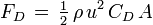
\includegraphics[width=3cm]{Ec1.png}\\
\end{center}
 
donde u es la magnitud del vector velocidad del objeto, CD es  el coeficiente de arraste (adimensional), A es el área transversal presentada por el objeto (sección eficaz). Por ejemplo, para una esfera el área transversal es A=pi*r , y  el coeficiente de arrastre es CD = 0.47.
 
Se pide agregar el efecto de resistencia del aire al objeto lanzado en tiro parabólico. El objeto ahora experimenta una fuerza de arrastre en la dirección del movimiento FD = FDx + FDy  o bien produciendo una aceleración variable aD = aDx + aDy = FD/m.
 
Modifica tu código Fortran para ahora incluir los efectos de fricción de arrastre por el aire. 

\begin{center}
	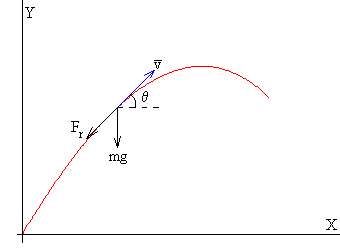
\includegraphics[width=10cm]{Im1.png}\\
\end{center}
 

\vspace{0.5cm}
La estructura del código debe contemplar lo siguiente:
 
1.Sección de declaración de variables

2.Sección de declaración de constantes

3.Subrutina para cálculo de trayectoria con entradas: dt, x0, y0, v0x, v0y, ax, ay; salida: t, x, y 

4.Subrutina para cálculo de fuerza de arrastre con entrada: m, densidad, A, CD, u0x, v0y ; salida: ax, ay

5.Se pide que utilizar un formato para escribir salida para los datos (ver ejemplo de formato):
              do i = 1, npts       
              write(1, 10001) x(i), y(i)
       end do 
  1001 format (2f10.6)
 

\vspace{0.5cm}
El código que usaremos será el siguiente:
\begin{verbatim}
Module constantes
implicit none
real, parameter :: dgt = (4.0*atan(1.0))/180
real, parameter :: pi = 4.0*atan(1.0)
integer, parameter :: npts = 6500

real, parameter :: aire = 1.29
real, parameter :: esfera = 0.47
real, parameter :: medesfera = 0.42
real, parameter :: cono = 0.5
real, parameter :: cubo = 1.05
real, parameter :: cuboa = 0.8
real, parameter :: cilindrol = 0.82
real, parameter :: cilindroc = 1.15
end module constantes

!~~~~~~~~~~~~~~~~~~~~~~~~~~~~~~~~~~~~~~~~~~~~~~~~~~~~~~~~~~~~~~~~~~~~~~~~~~~~~~~~~~~~~~~~~~~~

Subroutine confriccion (xini,yini,vini,angini,xmaxf,tf,ymaxf)
use constantes
implicit none
integer :: i
character :: object
real, dimension (0:npts) :: z,w,u,vz,vw,az,aw
real :: xini, yini, vini,angini
real :: xmaxf, ymaxf, tf
real :: ad,area,radio,cd,masa

Print *, "Ingresa la masa del cuerpo (kg) (reales)"
read *, masa
Print *, "Selecciona la masa del cuerpo"
Print *, "1.-Esfera"
Print *, "2.-Media esfera"
Print *, "3.-Cono"
Print *, "4.-Cubo"
Print *, "5.-Cubo angulado"
Print *, "6.-Cilindro largo"
Print *, "7.-Cilindro corto"
read *, object

Select case (object)
   case ("1")
      Print *, "Ingresa el radio de la esfera"
      read *, radio
      area = pi*radio*radio
      cd = esfera
   case ("2")
      Print *, "Ingresa el radio de la esfera"
      read *, radio
      area = pi*radio*radio*(1.0/2.0)
      cd = medesfera
   case ("3")
      Print *, "Ingresa el radio del cono"
      read *, radio
      area = pi*radio*radio*(1.0/3.0)
      cd = cono
   case ("4")
      Print *, "Ingresa la medida del lado del cubo"
      read *, radio
      area = radio*radio
      cd = cubo
   case ("5")
      Print *, "Ingresa la medida del lado del cubo"
      read *, radio
      area = radio*radio*sqrt(2.0)
      cd = cuboa
  case ("6")
      Print *, "Ingresa el radio del cilindro"
      read *, radio
      area = radio*radio*pi
      cd = cilindrol
   case ("7")
      Print *, "Ingresa el radio del cilindro"
      read *, radio
      area = radio*radio*pi
      cd = cilindroc
   case default
      Print *, "Error, comando no definido"
end select

z(0) = xini
w(0) = yini
vz(0) = vini*COS(angini)
vw(0) = vini*SIN(angini)
ad = (0.5*aire*area*cd)/masa
az(0) = -ad*vz(0)*vz(0)
aw(0) = 9.8-(ad*vw(0)*vw(0))
u(0) = 0

OPEN (2, FILE="confriccion.dat")
WRITE (2,1001) z(0),w(0)
1001 FORMAT (f11.5,f11.5)

DO i=0, npts, 1
  u(i+1) = u(i) + 0.01
  vz(i+1) = vz(i)+az(i)*u(i+1)
  vw(i+1) = vw(i)+aw(i)*u(i+1)
  az(i+1) = -ad*vz(i)*vz(i)
  aw(i+1) = -9.8-(ad*vz(i)*vz(i))
  z(i+1) = z(i)+vz(i)*u(i+1)+(0.5*az(i)*u(i+1)*u(i+1))
  w(i+1) = w(i)+vw(i)*u(i+1)+(0.5*aw(i)*u(i+1)*u(i+1))
  WRITE (2,*) z(i+1), w(i+1)
  IF (w(i)<0) EXIT
END DO
CLOSE (2)

xmaxf = z(i)
ymaxf = MAXVAL(w)
tf = u(i)*10.0

END SUBROUTINE confriccion

!~~~~~~~~~~~~~~~~~~~~~~~~~~~~~~~~~~~~~~~~~~~~~~~~~~~~~~~~~~~~~~~~~~~~~~~~~~~~~~~~~~~~~~~~~~~~~~~~

Subroutine sinfriccion (xini,yini,vini,angini,xmaxsf,ymaxsf,tsf)!use "sf" para simbolizar "sin friccion"
use constantes
implicit none
INTEGER :: i
Real, dimension (1:npts) :: x,y,t
REAL :: xini, yini, vini, angini   
REAL :: xmaxsf, ymaxsf, tsf    

angini=angini*dgt

xmaxsf = xini+((vini*vini+SIN(2*angini))/(9.8))
ymaxsf = yini+(((vini*vini)*(SIN(angini)*SIN(angini)))/(19.6))
tsf = (2*vini*SIN(angini))/(9.8)

open (1, file="sinfriccion.dat")

DO i=1, npts, 1
t(i)=FLOAT(i)*0.01
x(i) = xini + (vini*COS(angini)*t(i))
y(i) = yini + (vini*SIN(angini)*t(i)) - (4.9*t(i)*t(i))
WRITE (1,1001) x(i), y(i)
1001 FORMAT (f11.5,f11.5)
IF (y(i)<0) EXIT
END DO
CLOSE (1)

END SUBROUTINE sinfriccion

!~~~~~~~~~~~~~~~~~~~~~~~~~~~~~~~~~~~~~~~~~~~~~~~~~~~~~~~~~~~~~~~~~~~~~~~~~~~~~~~~~~~~~~~~~~~~~~

program projectilfriccion
use constantes  
       implicit none  
       real :: xini,yini,vini,angini
       real :: xmaxsf,ymaxsf,tsf,xmaxf,ymaxf,tf
       real :: diferencia 
       
       write(*,*) 'Ingresa la "x" inicial, la "y" inicial, la velocidad inicial, y el angulo inicial, respectivamente'   
       read *, xini, yini, vini, angini
   
       call sinfriccion (xini,yini,vini,angini,xmaxsf,ymaxsf,tsf)
       call confriccion  (xini,yini,vini,angini,xmaxf,ymaxf,tf)
       diferencia = ((xmaxsf-xmaxf)/xmaxf) * 100.0


write(*,*) '°~~~~~°~~~~~°~~~~~°~~~~~°~~~~~°~~~~~°~~~~~~°~~~~~°~~~~~°~~~~~°~~~~~°~~~~~°'
       write(*,*) 'Datos que usted ingreso:'
       write(*,*) 'Velocidad inicial:', vini,'m/s'
       write(*,*) 'Angulo de tiro:', angini,'radianes'
write(*,*) '.'
write(*,*) '.'
write(*,*) '.'
       write(*,*) 'Sin friccion'
       write(*,*) 'La altura maxima (y) es de: ', ymaxsf,'m'
       write(*,*) 'El tiempo total en el aire fue de:', tsf,'s'
       write(*,*) 'El alcance maximo (x) fue de:', xmaxsf,'m'
write(*,*) '.'
write(*,*) '.'
write(*,*) '.'
       write(*,*) 'Con friccion'
       write(*,*) 'La altura maxima (y) es de: ', ymaxf,'m'
       write(*,*) 'El tiempo total en el aire fue de:', tf,'s'
       write(*,*) 'El alcance maximo (x) fue de:', xmaxf,'m'
write(*,*) '.'
write(*,*) '.'
write(*,*) '.'
       write(*,*) 'La altura maxima (y) es de: La diferencia entre considerar y no considerar la friccion es de', diferencia,'%'
write(*,*) '°~~~~~°~~~~~°~~~~~°~~~~~°~~~~~°~~~~~°~~~~~~°~~~~~°~~~~~°~~~~~°~~~~~°~~~~~°'
  end program projectilfriccion 

\end{verbatim}

Ahora, verémos los resultados.

Primero se realizará una prueba lanzando una esfera de masa de 0.25kg, y radio de 0.05m, con un ángulo de 60° y desde el piso (0,0).
Los resultados que arroja el programa son los que aparecen en la siguiente imagen:


\begin{center}
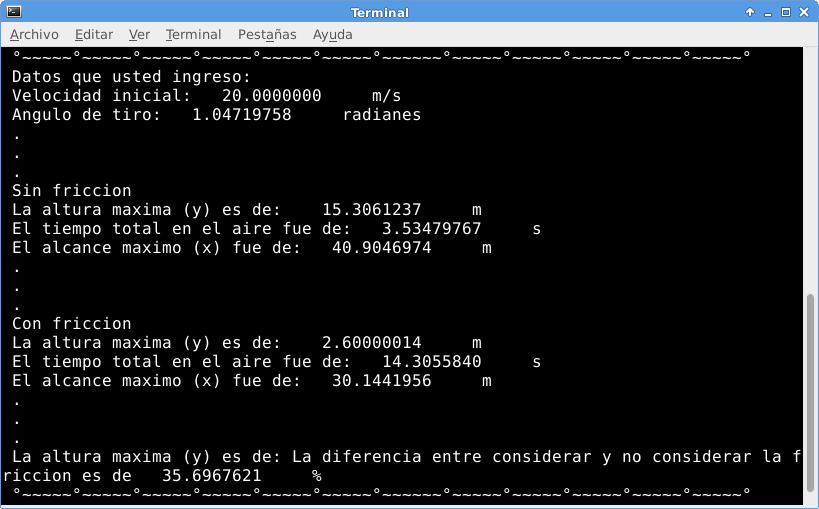
\includegraphics[width=15cm]{resul60.png}\\
\end{center}

Ahora, si pueden observar en el explorador de archivos, se crean dos archivos de datos, uno de el tiro con fricción, y el otro de el tiro sin fricción. Procedemos a graficar con gnuplot ambos tiros al mismo tiempo con el comando: $plot "confriccion.dat", "sinfriccion.dat"$. Nos saldrá la siguiente gráfica:

\begin{center}
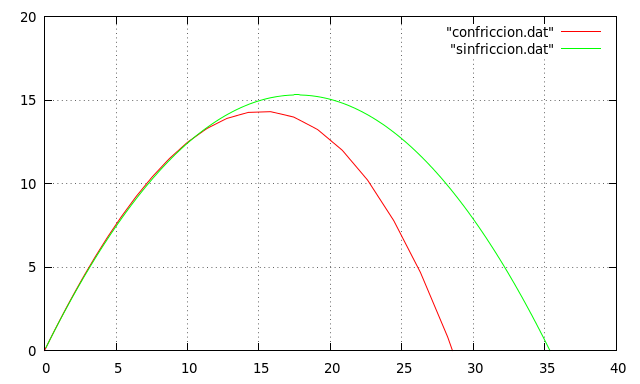
\includegraphics[width=15cm]{graf60.png}\\
\end{center}

Ahora, haremos la misma prueba, sólo que con 30 grados. Se pueden observar los siguientes resultados:


\begin{center}
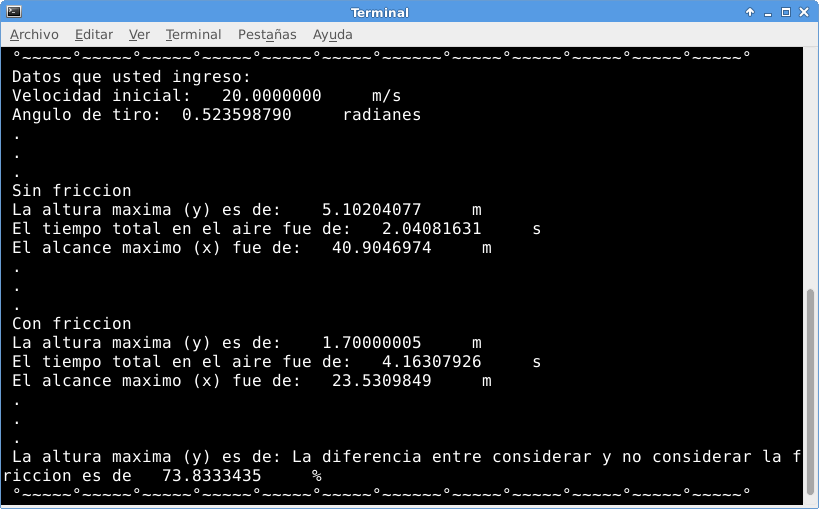
\includegraphics[width=15cm]{resul30.png}\\
\end{center}


\begin{center}
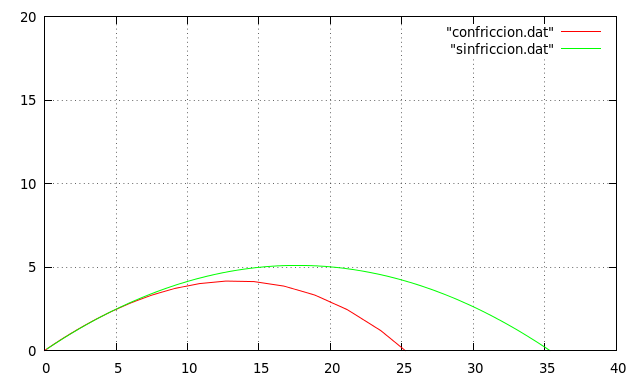
\includegraphics[width=15cm]{graf30.png}\\
\end{center}


Se puede observar que en el tiro sin fricción, los proyectiles de 60° y 30° caen en el mismo punto en x. Mientras que en el tiro con fricción, no sucede esto.

Aquí las cuatro gráficas juntas para una mejor comparación.

\begin{center}
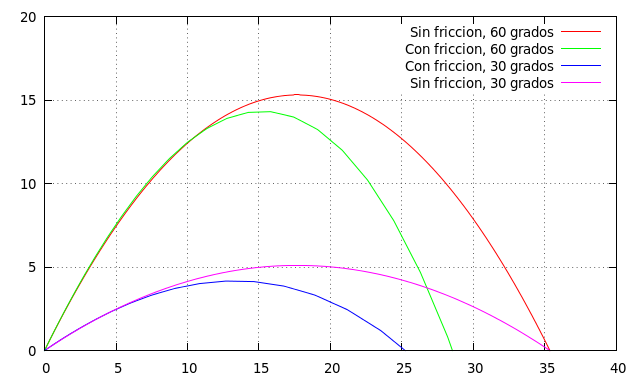
\includegraphics[width=15cm]{grafambos.png}\\
\end{center}



\end{document}
